
\documentclass[utf8,paper]{frontiersSCNS} % for Science, Engineering and Humanities and Social Sciences articles
\usepackage[utf8]{inputenc}
%\usepackage{inputenc}
\usepackage[english]{babel}
%\DeclareUnicodeCharacter{2264}{$\leq$}
%\DeclareUnicodeCharacter{002E}{$\leq$}
\usepackage{letltxmacro}

\usepackage{stringenc}
\usepackage{pdfescape}

\makeatletter
%\renewcommand*{\UTFviii@defined}[1]{%
%  \ifx#1\relax
%    \begingroup
%      % Remove prefix "\u8:"
%      \def\x##1:{}%
%      % Extract Unicode char from command name
%      % (utf8.def does not support surrogates)
%      \edef\x{\expandafter\x\string#1}%
%      \StringEncodingConvert\x\x{utf8}{utf16be}% convert to UTF-16BE
%      % Hexadecimal representation
%      \EdefEscapeHex\x\x
%      % Enhanced error message
%      \PackageError{inputenc}{Unicode\space char\space \string#1\space
%                              (U+\x)\MessageBreak
%                              not\space set\space up\space
%                              for\space use\space with\space LaTeX}\@eha
%    \endgroup
%  \else\expandafter
%    #1%
%  \fi
%}
\makeatother

\LetLtxMacro{\ORIGselectlanguage}{\selectlanguage}
\makeatletter
\DeclareRobustCommand{\selectlanguage}[1]{%
  \@ifundefined{alias@\string#1}
    {\ORIGselectlanguage{#1}}
    {\begingroup\edef\x{\endgroup
       \noexpand\ORIGselectlanguage{\@nameuse{alias@#1}}}\x}%
}
\newcommand{\definelanguagealias}[2]{%
  \@namedef{alias@#1}{#2}%
}
\makeatother

\definelanguagealias{eng}{english}
\definelanguagealias{en}{english}

\makeatletter
\let\l@eng\l@english
\makeatother

%\setcitestyle{square}
\usepackage{url,hyperref,lineno,microtype}
\usepackage[onehalfspacing]{setspace}
%\linenumbers


% Leave a blank line between paragraphs instead of using \\


\def\keyFont{\fontsize{8}{11}\helveticabold }
\def\firstAuthorLast{Diego Angulo {et~al.}} %use et al only if is more than 1 author
\def\Authors{Diego Andres Angulo\,$^{1,*}$, Jose Tiberio Hernandez\,$^{1}$ , James Oliver$^{2}$ and Cyril Schneider\,$^{3}$}
% Affiliations should be keyed to the author's name with superscript numbers and be listed as follows: Laboratory, Institute, Department, Organization, City, State abbreviation (USA, Canada, Australia), and Country (without detailed address information such as city zip codes or street names).
% If one of the authors has a change of address, list the new address below the correspondence details using a superscript symbol and use the same symbol to indicate the author in the author list.
\def\Address{$^{1}$ IMAGINE, Universidad de los Andes, Bogotá , Colombia \\
$^{2}$VRAC, Iowa State University, Ames , IA, Unites States
\\
$^{3}$CNS, CHUL, Quebec , QC, Canada  }
% The Corresponding Author should be marked with an asterisk
% Provide the exact contact address (this time including street name and city zip code) and email of the corresponding author
\def\corrAuthor{Diego A. Angulo}
\def\corrAddress{IMAGINE, Universidad de los Andes, Carrera 1 \# 18A -12 , Bogotá, Colombia}
\def\corrEmail{da.angulo39@uniandes.edu.co}

\begin{document}
\onecolumn
\firstpage{1}

\title[Braviz]{Braviz: Visual Exploratory Analysis of Brain Datasets} 

\author[\firstAuthorLast ]{\Authors} %This field will be automatically populated
\address{} %This field will be automatically populated
\correspondance{} %This field will be automatically populated

\extraAuth{}% If there are more than 1 corresponding author, comment this line and uncomment the next one.
%\extraAuth{corresponding Author2 \\ Laboratory X2, Institute X2, Department X2, Organization X2, Street X2, City X2 , State XX2 (only USA, Canada and Australia), Zip Code2, X2 Country X2, email2@uni2.edu}

\maketitle

%%%%%%%%%%%%%%%%%%%%%%%%%%%%%%%%%%%%%%%%%%%%%%%%%%%%%%%%%%%%%%%%%%%%%%%%%%%%%%%%%%%%%%%%%%%%%%%%%%%%%%%%%%%%%%%%%%%%%%%%%%%%%%%%%%%%%%%%%%%%%%%%%%%%%%%%%%%%%%%%%%%%%%%%%%%%%%%%%%%%%%%%%%%%%%%%%%%%%%%%%%%%%%%%%%%%%%%%%%%%%%%%%%%%%%%
%%% The sections below are for reference only.
%%%
%%% For Original Research Articles, Clinical Trial Articles, and Technology Reports the section headings should be those appropriate for your field and the research itself. It is recommended to organize your manuscript in the
%%% following sections or their equivalents for your field:
%%% Abstract, Introduction, Material and Methods, Results, and Discussion.
%%% Please note that the Material and Methods section can be placed in any of the following ways: before Results, before Discussion or after Discussion.
%%%
%%%For information about Clinical Trial Registration, please go to http://www.frontiersin.org/about/AuthorGuidelines#ClinicalTrialRegistration
%%%
%%% For Clinical Case Studies the following sections are mandatory: Abstract, Introduction, Background, Discussion, and Concluding Remarks.
%%%
%%% For all other article types there are no mandatory sections.
%%%%%%%%%%%%%%%%%%%%%%%%%%%%%%%%%%%%%%%%%%%%%%%%%%%%%%%%%%%%%%%%%%%%%%%%%%%%%%%%%%%%%%%%%%%%%%%%%%%%%%%%%%%%%%%%%%%%%%%%%%%%%%%%%%%%%%%%%%%%%%%%%%%%%%%%%%%%%%%%%%%%%%%%%%%%%%%%%%%%%%%%%%%%%%%%%%%%%%%%%%%%%%%%%%%%%%%%%%%%%%%%%%%%%%%

\begin{abstract}

%%% Leave the Abstract empty if your article falls under any of the following categories: Editorial Book Review, Commentary, Field Grand Challenge, Opinion or specialty Grand Challenge.
\section{}
Brain researchers typically deal with large amounts of data from different sources and often, of different nature. This requires the use of several different software tools and makes it cumbersome and time consuming to answer simple questions. Because of this, data is not used to its fullest potential, and exploratory analysis is rarely done . This paper presents a software tool called BRAVIZ that integrates access to several data types and automates many of the cumbersome and error-prone tasks required to explore typical neuroscience data. This work focuses on integrating interactive visualization with real-time statistical analyses to facilitate exploration and discovery. BRAVIZ enables an inversion of the typical neuroscience analysis process by emphasizing images as the main organizing objects in the process rather than relying in abstract numerical indicators. This encourages researchers to notice trends and relationships, which motivate additional analyses and generally gain a fuller understanding of the phenomena represented by the data.  A case study is presented that incorporates MRI, DTI, and fMRI images together with a large amount of neuro-psychological and clinical data.  The case study demonstrates how BRAVIZ enables researchers to discover new hypotheses about the relationships between structure and functions of the brain.

\tiny
 \keyFont{ \section{Keywords:} Exploratory Analysis, Visual Analytics, Brain Data, MRI, Tractography, Cohorts } %All article types: you may provide up to 8 keywords; at least 5 are mandatory.
\end{abstract}



%%%%%%%%%%%%%%%%%%%%%%%%%%%%%%%%%%%%%
%From Cyril
% The 3 sections that precedes are not clear for me and should be re-written following my suggestions in order for the text to be stronger – there is no line of thoughts (at least for me, it’s very difficult to follow the ideas with all back and forth passages – especially, some passages are not correctly located (I mean, not in the right section). I may propose to point out the requirement of exploratory analysis and what is missing currently in literature and to state that Braviz will respond to these needs by cumulating the advantages of other techniques / softwares but avoiding the disadvantages (for example by creating an interface for the different tools interplay) – this provides the transition for presenting the tools. Be careful, this presentation is not for free and shall respond to a need.
%%%%%%%%%%%%%%%%%%%%%%%%%%%%%%%%%%%%%%%%%%%%%%%%%

% Intro
% Requirements for exploratory analysis

% Related Work
% What is missing currently in literature

% Presentation, all justified on objectives, nothing is free
% Braviz... accumulates advantages and avoids disadvantages


\section{Introduction}

An important challenge in addressing how brain works in normal but also pathological conditions and how it reorganizes  requires to understand the extent to which the physical structure of brain underlies the way it functions. The most common research procedure is characterized by the conduction of experiments aiming at collecting data directed towards testing a former hypothesis. This  confirmatory-like methodology imposes limitations on the way data is used, and especially the outcomes collected one time only which is unfortunate owing to the fact that data acquisition is time and resources consuming.

Structural information is gathered mainly through the use of imaging techniques such as Magnetic Resonance Imaging (MRI), Computer Aided Tomography (CAT) or Positron Emission Tomography (PET). Other methods measure the electrical activity of the brain, as in Electro-Encephalography (EEG) or Magneto-Encephalography (MEG). Transcranial Magnetic Stimulation (TMS) is a technique that stimulates cells using a rapidly changing magnetic field that generates an electrical field in the neurons. For example, stimulating the motor cortex will produce an electrical signal on the muscles that can be registered using electro-myography (EMG). These has to be combined with clinical and neuro-psychological data in order to relate structure with function.
										
In the two last decades data has been gathered in a more open fashion with the availability of more and more public databases on brain research data. Additionally, rapid improvements are underway in the way data is collected, stored and shared, both at the technical and policy levels (see \cite{eckersley_neuroscience_2003}). These allows massive amounts of data to be consolidated into databases and searched in efficient ways. In this ways questions can be explored first with already acquired data, and large data pools can be mined for interesting relationships. This is leading to a change in the way research is done. This is, a shift from hypothesis driven research into data driven research, where data is available before questions and hypotheses, and these are raised based on the data.
				
The methodology used in data driven research differs significantly from the one in hypothesis driven research. The process of extracting meaningful insights from a data-set is known as exploratory research. It involves iterating through data several times, looking at it from different points of view, searching for relevant subjects and measures, gathering details from individuals and performing group analyzes involving different measures. These are just some of the analysis tasks that make part of exploratory research. These are carried out multiple times in different order as researchers learn more about the data-set. 

During this process several patterns will appear in the data which could lead to new unexpected insights. Unfortunately, it is also likely that these patterns are caused by peculiarities of the current data-set and can't be generalized outside of it. Automatic data-mining algorithms can find thousand of possible relations, but true findings need to be backed up by science and current knowledge. Therefore interpretation of insights must be done by domain experts. In addition, insights that integrate data from different domains have to be analyzed by experts with experience in these domains. 

Current tools are specialized in particular data types, and are optimized to support linear work flows. In order to integrate data from different domains and to perform different analysis tasks, experts have to switch between tools  and in the worst cases they even have to move to a different computer. Under this conditions, an efficient integrated exploratory analysis is not feasible. 

					
Similar scenarios have appeared in other domains, such as in economics, terrorism prevention and business intelligence (see \cite{cook_illuminating_2005}). The common challenge is extracting meaningful insights from large and heterogeneous data-sets. In these scenarios, systems that combine statistics, machine learning, and data mining; together with interactive data visualization allow analysts to take decisions supported by data. 

Visual analytics \citep{keim_visual_2008} has emerged as a discipline which attempts to integrate all of these areas with the objective of making optimal use of the available data. The analyst is acknowledged as the most important actor in visual analytics, and all tools should be there to support him, and provide him timely access with the required data and tools. It is crucial that these tools behave in intuitive ways, so analysts can keep their full attention on the data and don't get distracted by details of the tools. 
					
In data driven brain research, researchers can also benefit from these techniques. Data sets are likely to contain a combination of structural and clinical data. Structural data is initially acquired as images with different contrasts. For example MRI machines can be used to acquire anatomical images, diffusion weighted images (DWI) and functional images (fMRI) among others. These images can be processed in specialized tools to produce structures segmentations and reconstructions, reconstruction of white-matter pathways, statistical maps representing the involvement of brain areas in particular tasks, and connectivity networks. These has to be combined with clinical and neuro-pshychological data; and the whole set is the input for exploratory analyzis.


This paper introduces BRAVIZ, a tool based on visual analytics aimed at supporting exploratory analysis in brain research. Most specifically, the tool is centered at data-sets which integrates MRI derived data with clinical and socio-economic data. It includes several small applications designed to support concrete analysis tasks, but which can be used together to support full exploratory analyses. This environment allow researchers to find answers to questions inside the data-set, as well as explore the data-set in order to discover interesting patterns and trends. This exploration is carried out through different interactive visualizations, combined with mechanisms to filter subjects, dig down for details, and data aggregation.


\section{Related Work}

Several tools have been developed to support research based on neuro-images. However most of them are optimized for the linear workflow found typical of confirmatory analyzes, and they are cumbersome to use for exploratory analyzes or data-driven research.

For example, Freesurfer  \citep{fischl_freesurfer_2012}, fsl\citep{jenkinson_fsl_2012} and spm \citep{friston_statistical_2006} can be used to segment, register and perform statistical testing of image data. 3D slicer \citep{fedorov_3d_2012}, Brain Visa \citep{cointepas_brainvisa:_2001} and ITKSnap \citep{yushkevich_user-guided_2006} are other commonly used tools which allow integration of data from different image modalities. These tools are efficient at processing bulk images in a pipeline, but they fall short when several iterations through the data are required. The interfaces for statistical hypothesis testing require extensive configuration, which is appropriate for testing selected hypotheses, but becomes cumbersome for trying several combinations. Efficient mechanisms for filtering the subjects list after the analysis, or going back to the details of a particular subject from group results are not included. Complementary data loaded from tables can be used, but changing variables often means creating new tables and adjusting them the required format.

Information visualization tools like ggobi\citep{cook_interactive_2007}, aabel, SPSS, stata and Tableau\citep{hanrahan_tableau_2003} can be used for interactive exploration of a data-set. These tools permit data transformation, model fitting, and interactive visualization. Through them user may detect outliers and interesting subgroups, and grasp subtle patterns and trends. However these tools only support tabular data. Scalar data derived from images can be added, but there is no easy way to link to the original data, or to examine spatial features that can't be encoded into variables. 

INVIZIAN \citep{bowman_query-based_2011,bowman_feature-similarity_2012,bowman_visual_2012} is an application for exploring large brain data-sets which integrates structural and scalar data. It organizes data in an abstract 3D space in such a way that similar brains are located close to one another. It integrates with ggobi to explore relations between scalar values and spatial brain features. However, this tool only deals with structural MRI, and the proposed workflow is automatic extraction of scalar features from such images. This is not appropriate for the target study, as it has several image modalities, and the focus is on visually finding patterns and trends based on the expertise from the users rather than by using machine learning algorithms. Notice both approaches are complementary.

In \citep{hinterberg_peax:_2014} a visual analysis tool for high dimensional data. It lets the user quickly iterate through several models and try different parameters. The model is displayed visually together with distributions of the selected parameters, and there are tools available to filter out the set of possible parameters. This tool is also optimized for a single type of data, a single type of model and an specific workflow. The BRAVIZ proposal seeks to support multiple tasks and workflows by providing a set of applications, which can be used independently or combined to perform complex analyzes. It attempts to bring clinical data and tools from the information visualization domain closer to the neuroimage domain, in such a way that they can be used by experts from different areas working as a team.

Even though multiple tools exist for analysis and exploration of spatial and non-spatial data, it is still a challenge to integrate multiple kinds of analyzes and multiple kinds of data in a single environment. This causes researchers to spend significant time moving data from tool to tool, and additionally they are required to learn different tools with different interaction models. BRAVIZ provides a unified environment for analyzing spatial and non-spatial data. It leverages existing algorithms and exposes them through  consistent interface. This provides an environment that lets researchers explore and manipulate data efficiently.

\section{Proposed Environment}


Instead of a monolithic application, BRAVIZ is a set of small applications that solve specific analysis tasks, and a library which abstracts common operations (see Figure \ref{fig_arch}). This divisions permits application developers to focus on the high level operations required to support the analysis tasks, while data management and processing problems are solved only once inside the common library. 

\subsection{Design and Development Methodology}

A ``user centered'' approach\citep{fernandez_user-centered_2013,wassink_applying_2009} was used. The authors worked closely with brain researchers of several specialties, visited several labs and hospitals, and learned as much as possible about typical neuroscience research workflows and the bottlenecks they contain. The design, development and evaluation process consisted of several iterative cycles, prototypes were shared with domain experts, and their feedback motivated design ideas and usability enhancements for the next generation. As the development cycles progressed, the domain experts ventured further away from common paradigms.

The initial stages of design focused on identifying the obstacles that affected communication between experts, and explored ways of mitigating them. The team of experts was composed of radiologists, psychiatrists, pediatricians, physicians, physiologists, neonatologists,  statisticians, engineers and economists. This effort exposed typical process bottlenecks that affect efficient exploratory analyzes. By decreasing data access overhead, BRAVIZ accelerates exploratory research and gives experts access to data that is typically out of their area of expertise.

An extensive literature review of studies with data similar to that of the Kangaroo study, led to better understanding of the kinds of data patterns and relationships researchers look for. In addition, the data visualizations in these publications were the basis for BRAVIZ visualizations, given that most researchers are familiar with them. From analyzing the visualization capabilities in current neuro-image tools, as well as how experts use them, the BRAVIZ team learned what was expected from image viewers, which features were important and which ones were seldom used. Tools like SPM \citep{friston_statistical_2007}, Osirix \citep{rosset_osirix:_2004} and 3D-Slicer \citep{fedorov_3d_2012} were the reference for this stage. For example, it is very important for researchers to visualize several types of data in the same space, and to be able to compare two images together. It was also evident that there is a need to integrate spatial visualizations with non spatial data about the same subject, as usually researchers need to open two different applications. It was also evident the need for moving across subjects in the study, without having to start from zero each time. Most applications include command line interfaces, but our target users prefer graphical user interfaces. 

\subsection{Solution Structure}

The set of applications that make up BRAVIZ provides different views on the same data-platform, which provides structured access to spatial and non-spatial data. It stores pre-processed spatial data together with registration transforms allowing integrated access to images, tratographies, models and statistical maps in integrated coordinate systems. Non-spatial data is stored as variables with complimentary meta-data, which allows a more meaningful usage throughout the applications. This platform also holds sub-samples, geometric objects and visualizations defined by the researchers as they explore. 

All of these are available to any tool, but each tool will focus on different types of data on different contexts. Therefore, even though each application is tailored to specific tasks, several applications can be used together to solve more complex problems. Additionally, applications can share information in real-time without going through the database, this for example, allows researchers to focus on the same subject from all applications. The system keeps a log of user interaction and permits revisiting any state. This history can be further annotated by adding comments and highlighting the most relevant steps.

Currently, BRAVIZ includes tools to look at spatial data from a single subject with high detail, as well as tools to look at spatial data associated with a sub-sample; both with numerical and categorical data as context. Several tools for visualizing and working with non-spatial data are also included, which provide scatter-plots, box-plots, histograms and other visualizations centered around an analysis tasks. These visualizations are interactive and capable of generating a dialogue with the user.
As Colin Ware \citep{ware_information_2004} said ``The best visualizations are not static images to be printed in books, but fluid, dynamic artefacts that respond to the need for different views or for more detailed information''. In all non-spatial visualizations users can select individual points, and open additional details of the specific subjects in other applications. 

By having different points of view, researchers can get a more complete picture of each subject. In addition, different researchers can focus their work on specific analysis tasks, while making their results available for the rest of the team. Researchers can also review a particular line of thought from themselves or colleagues in order to better understand finding and propose future directions. Altogether, the system is meant to provide quick access to data and algorithms and therefore support the exploratory analysis cycle. 

\subsection{Applications Set}

%Not sure if this needs a different section, maybe it should be summarized into the description

The current set of applications comprising BRAVIZ can be divided in three categories. One set of applications focuses on measuring or creating new descriptors from geometric data, another focuses on displaying geometric data using other variables as context, and the last one focuses on exploring numerical and categorical data while maintaining a link to the underlying geometric data. These applications mainly support different stages of the exploratory analysis process, respectively, data transformation, visualization and modeling. Notice that these stages may be visited several times in different orders during an analysis session.

Additionally there are utilities for importing and exporting data in spreadsheet format; so that the tools can interact with third party statistical software. All tools are accessible from the graphical menu shown in figure \ref{fig_menu}. The applications included in the current version are listed below, followed by an extended description of three of them.

\begin{itemize}
\item Create and Measure: Define new scalars based on spatial data for the whole cohort.
\begin{itemize}
\item Roi Builder: Create spherical regions of interest, using images or surfaces as context.
\item Linear Measure: Measure elements of any image using lines
\item Logic Bundles: Define fiber bundles through logical operations on ROIs and segmented structures.
\end{itemize}
\item Visualize Spatial Data: Explore and analyze spatial data.
\begin{itemize}
\item Subject Overview: Visualize several spatial objects in the same space, as well as context information for a single subject.
\item Sample Overview: Repeat the same visualization for a group of subjects, sorted by a numerical variable and divided in groups by a nominal variable.
\item Explore fMRI: Visualize BOLD time-lines, experiment design and contrasts.
\item Check Registration: Visualize two images together to evaluate the quality of registration. 
\end{itemize}
\item Visualize non-spatial data
\begin{itemize}
\item Anova : Perform ANOVA analyzes using the database variables.
\item Linear Model: Fit a linear model to variables in the database.
\item Correlations: Explore correlations between variables in the database.
\item Parallel Coordinates: Visualize multiple variables in interactive parallel coordinates.
\end{itemize}
\end{itemize} 

The main interface of the Subject Overview application is shown on Figure \ref{fig_subject}. This tool provides access to MRI Images, Freesurfer segmentations and cortex reconstructions, deterministic tractography, tracula bundles and fMRI statistical maps. Some geometrical features, as volume or mean FA inside a structure, can be captured directly from  this application and added into the database as a new variable. Below the main view  is a context panel, that displays the values of selected variables for the current subject. To change the current subject the user may use the controls underneath the main view, or select from the table in the subjects panel at the left. All of the current selected variables and geometric objects in the view are updated to display the information for the new subject. Thus it is straightforward to look at a certain aspect across different subjects. In the lower left corner is a control that allows the user to select between native subject MRI coordinate systems, a Talairach linear registration or a Dartel non linear registration. These features allow efficient exploration of spatial characteristics from different subjects.

A small-multiples view\citep{tufte_visual_1983} display of several subjects (see Figure \ref{fig_sample}), is available in the Sample Overview application. This application is useful for finding trends across a sample or doing quality control and spotting problematic images. Subjects are arranged from left to right according to a numerical variable, and rows are defined by a nominal variable. In the example shown the two rows are males and females, and the ordering variable is the score in a math test. The bar-plot at the right shows the distribution of the variable among the two groups and is linked with the 3d views. The configuration of 3d viewers is copied from Subject Overview, in this way the interface is kept simple, as there is no need for visual configuration options.

The Anova application (see Figure\ref{fig_anova}) was developed to support fast Anova modeling using the variables in the database. In order to perform the analysis the user must select an outcome variable, one or more regressors and interaction terms, and a sub-sample.  Then the user clicks the \emph{Calculate Anova button}, which fetchs the required data from the database and performs the calculation. The main plot will show diagnostics, i.e. distribution of residuals and a scatter plot of residuals vs fitted values, and the table at the bottom right shows the resulting fitted values. By double clicking on any tabñe row a plot showing the effect of that particular term will be displayed. 

Figure \ref{fig_other_apps} shows other applications currently built into the system. For additional information about how the system is implemented please refer to the additional material.

\section{Case Studies}

In this research, a particularly representative case study, the kmc project \citep{schneider_cerebral_2012}, is introduced to both motivate the requirements for BRAVIZ and demonstrate its effectiveness. The kmc study explores the effect of treatment options on premature births and data on subjects was collected from several fronts. The original randomized study involving about 750 preterm babies was conducted in 1994 \citep{charpak_kangaroo_1997}. These kids were followed during their first year \citep{charpak_randomized_2001, tessier_kangaroo_2009} of life and several clinical and socio-economical variables were registered. Forty of the kids from the original study were re located at fifteen years of age, the  subjects went through several neuro-psychological tests, measuring attention, memory, reasoning skills and hand-eye coordination among others. They also went to vision, hearing and full medical examinations. Finally, they were scanned with Structural MRI, DTI and several fMRI protocols. \footnote{agregar este protocolo} These images were processed using freesurfer \citep{fischl_freesurfer_2012}, fsl\citep{jenkinson_fsl_2012}, camino\citep{cook_camino:_2006}, and spm\citep{friston_statistical_2006}; which extracted several numerical measurements and geometric structures as segmentations and tractographies. All of this data was collected for testing specific hypotheses but the specialists involved in the study are also interested in analyzing it for unexpected relationships and trends; in other words, to perform an exploratory analysis\citep{tukey_we_1980}.

\section{Discussion}
\label{sec:disc}
%Several users who have contributed to the development of BRAVIZ now use it regularly as part of their work. They continue experimenting with the tool and proposing improvements. Many users, especially those without expertise in image processing, like how they now can create and analyze spatial data on their own.  By using BRAVIZ it is straightforward to explore the data and answer questions. It is also common for more complex ideas to occur to the user while exploring. While exploring in this fashion, experts often discover new ways to use the processing power of tools like Freesurfer or SPM; and therefore take better advantage of them.
%
%Even without looking at spatial data, users enjoy getting visualizations of nominal and numerical variables instantaneously, which allows them to explore the dataset efficiently. BRAVIZ tools have proven to be easy to learn. It is designed to provide a starting point for facilitating exploratory analysis, and we expect that afterward users may move to more powerful and complex tools.
%
%The features that BRAVIZ users appreciated the most were quick identification of outliers and being able to find nominal and numerical data together with the corresponding image data. An unexpected result was that by exploring the data with BRAVIZ several data problems were discovered and many of them could be fixed by going back to the raw data or processing again. 
%
%The examples shown here used a rather small database, but BRAVIZ has been used successfully in a similar study with around 400 subjects. At this scale most of the visualizations still work, but for larger datasets new approaches must be developed. 
%
%Some researchers are used to working only in confirmatory analyses, and are very cautious about exploring data freely. Sometimes they fear that exploration might invalidate any chance of publishing results. However as long as care is taken on interpreting the results of exploration and hypotheses are tested on independent datasets there is no danger in doing exploratory analyses. It is well known that the amount of data available for analysis today is enormous, but better tools are needed to navigate and explore it. There is also an opportunity to change workflows to adjust to this new reality and take the best advantage of the available data. Data mining tools and visual exploration of data has been successfully applied in several other areas, such as business and law enforcement, and will continue to gain popularity in brain research. 
%
%Collaboration between experts is improved by having visualizations available to explain ideas. By having several applications open, large display real-estate can be leveraged (see Figure \ref{fig_imagine}). This works best when several experts are looking from different perspectives, and in this way unexpected elements and multidimensional trends can be spotted.
%
%%Future work
%%Web based?
%
%In its current state BRAVIZ runs on the user's machine, and the installation process is not trivial. In the future it should transform into a webservice, running no a cloud environment, and available through a standard web-browser. However, the technology for displaying interactive 3D images on a web environment is not mature enough. Nevertheless, technologies as Brainbrowser\citep{sherif_brainbrowser:_2014}, and paraview\citep{ahrens_36_2005} are advancing fast, and probably in the near future it will be able to migrate to such a platform. 

% Though the system is built from several small applications, they are designed to work together synchronously in order to support more complex tasks. Subsamples, variables and subjects of interest can be shared across tools and among colleagues. Altogether, this creates a flexible environment that can be adapted to several kinds of data, questions, workflows and experts. These features, combined with having all data and analysis tools a couple of clicks away; provides a pleasant and efficient exploratory analysis environment. 


\bibliographystyle{frontiersinSCNS_ENG_HUMS} % for Science, Engineering and Humanities and Social Sciences articles, for Humanities and Social Sciences articles please include page numbers in the in-text citations
%\bibliographystyle{frontiersinHLTH&FPHY} % for Health and Physics articles
\bibliography{zotero}

%%% Upload the *bib file along with the *tex file and PDF on submission if the bibliography is not in the main *tex file

\section*{Implementation (Appendix)}

BRAVIZ is implemented in Python, a popular language in the neuroscience community \citep{gorgolewski_nipype:_2011, garyfallidis_dipy_2014}.  Powerful plotting, rendering, and data manipulation libraries are available. The trade-off is a loss of performance compared to compiled languages, but so far interactivity has been maintained by letting VTK\citep{schroeder_vtk_1998} and Numpy\citep{van_der_walt_numpy_2011} do the most intensive operations. It has been tested in Mac, Windows and Linux.

BRAVIZ is also a library that can be used for creating custom interactive visualizations that support specific tasks. Figure \ref{fig_arch} shows the general architecture. The library abstracts functionality that is common to several applications, allowing applications designers to focus on providing a fluid experience for the user.

The ``Read and Filter'' module handles all access to the file system or network. Each BRAVIZ project is composed of a SQLite database, and spatial data. This module provides other useful functions like attaching scalars to geometric objects, filtering fiber bundles and transforming between coordinate systems. Underneath it relies heavily on nibabel\citep{gorgolewski_nipype:_2011}, numpy\citep{van_der_walt_numpy_2011} , scipy\citep{jones_scipy:_2001,oliphant_python_2007} and VTK\citep{schroeder_vtk_1998} . Notice that this module handles all the necessary transformations of spatial data, and exposes a high level interface to the upper layers. In this way application designers can focus on visualization and interaction as required by end users and let the library handle registration and other low level operations. The module also provides access to numerical and categorical variables that are stored in a database. Pandas' DataFrames\citep{mckinney_data_2010} are the preferred way to manipulate this data. The database also holds annotations, scenarios, user defined geometrical objects and analysis history. 

Specific project reader modules can be created to adjust to the layout, file names and other peculiarities of each research project. The active project, favorite variables and favorite subject and other preferences are specified through a configuration file.
By accessing data through this module, developers can create applications that can be reused in several projects. 

The ``visualization'' module provides reusable components for visualizing spatial and non-spatial data. VTK is used for all the 3D visualization while 2D visualization is achieved through matplotlib \citep{hunter_matplotlib:_2007} and seaborn\citep{michael_waskom_seaborn:_2014} in native applications, or through D3 \citep{bostock_d3_2011} in web applications.

The ``interaction'' module contains, among others, several reusable user interface components, functions for doing statistical calculations in R\citep{team_r:_2012, gautier_rpy2:_2008} and additional processing for geometric data, and connection mechanisms between applications. The current version uses PyQt4 for the user interface with some web based visualizations built using the tornado framework \citep{server_source_2008}. 

Individual applications use a different mixture of the provided modules depending on user requirements. Most of the code inside each application should be about user interaction and coordination between visualizations. If new data processing algorithms or visualizations are required they should be implemented as reusable components in the library so that future applications can benefit from them. The project is licensed under a lesser general public license (LGPL) and its source code is available at \url{https://bitbucket.org/dieg0020/braviz}, together with installation instructions. Additional documentation is available at \url{http://diego0020.github.io/braviz}.

\section*{Acknowledgments}

\section*{Figures}

%%% Use this if adding the figures directly in the mansucript, if so, please remember to also upload the files when submitting your article
%%% There is no need for adding the file termination, as long as you indicate where the file is saved. In the examples below the files (logo1.jpg and logo2.eps) are in the Frontiers LaTeX folder
%%% If using *.tif files convert them to .jpg or .png
\begin{figure}[h!]
\begin{center}
\includegraphics[width=0.4\textwidth]{figures/braviz_menu.PNG}
\end{center}
 \textbf{\refstepcounter{figure}\label{fig_menu} Figure \arabic{figure}.}{This menu is currently used to access the different applications. It also provides facilities to review the available variables and the saved scenarios, to view and create subsamples, and to import to and export from spreadsheets.  }
\end{figure}

\begin{figure}[h!]
\begin{center}
\includegraphics[width=0.9\textwidth]{figures/subj_overview_full.PNG}
\end{center}
 \textbf{\refstepcounter{figure}\label{fig_subject} Figure \arabic{figure}.}{Main interface of the subject overview application. At the bottom of the render panel some variables about the subject are shown to provide context. At the bottom-left corner we have controls to change the coordinate system, and to move the camera to preset positions. Most of the data is available via the different tabs at the left panel. The current tab provides a list of available subjects, it is enough to double click in a row to get the selected data for that subject. The arrows directly under the 3D viewer provide another convenient way to move through the subjects following the order of the list. }
\end{figure}

\begin{figure}[h!]
\begin{center}
\includegraphics[width=0.9\textwidth]{figures/sample_overview.PNG}
\end{center}
 \textbf{\refstepcounter{figure}\label{fig_sample} Figure \arabic{figure}.}{This application gives access to the data of several subjects at the same time. Images are sorted from left to right according to a numerical variable (shown in the bars at the right) and arranged in columns by a cathegorical variable (bars color)  }
\end{figure}

\begin{figure}[h!]
\begin{center}
\includegraphics[width=0.9\textwidth]{figures/anova.PNG}
\end{center}
 \textbf{\refstepcounter{figure}\label{fig_anova} Figure \arabic{figure}.}{An application for performing ANOVA analyses using the data in the BRAVIZ database. You can right click on an outlier to select it on all open BRAVIZ applications. }
\end{figure}

\begin{figure}[h!]
\begin{center}
\includegraphics[width=0.9\textwidth]{figures/many_apps.png}
\end{center}
 \textbf{\refstepcounter{figure}\label{fig_other_apps} Figure \arabic{figure}.}{Examples of currently available applications. A) ROI builder. B) Linear model. C) Explore fMRI. D) Correlations. E) Parallel coordinates}
\end{figure}

\begin{figure}[h!]
\begin{center}
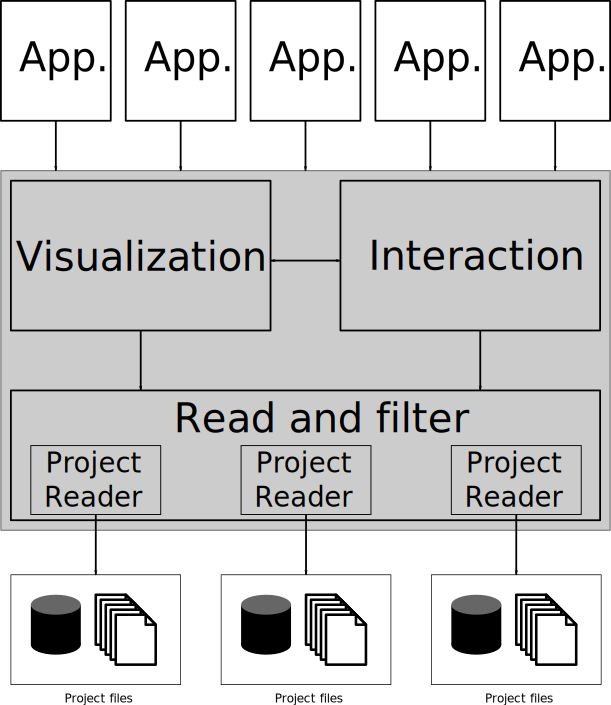
\includegraphics[width=0.4\textwidth]{figures/arquitecture.png}
\end{center}
 \textbf{\refstepcounter{figure}\label{fig_arch} Figure \arabic{figure}.}{The BRAVIZ software architecture. At the bottom there are specialized reader classes for each data-set which handles low level access to the specific projects' data. In gray is the main  library, which provides modules for visualization, interaction and data manipulation. On top user applications are built. In order to adapt the system to a new data-set it is only necessary to adapt a project reader.}
\end{figure}

\begin{figure}[h!]
\begin{center}
\includegraphics[width=0.9\textwidth]{figures/imagine.jpg}
\end{center}
 \textbf{\refstepcounter{figure}\label{fig_imagine} Figure \arabic{figure}.}{An example of BRAVIZ running on a large display in a collaborative setting. All of the applications are linked, this means that selecting a subject in one application will highlight or select that subject on all of them.}
\end{figure}




\end{document}
